\documentclass[a4paper, 11pt]{article}
\usepackage[english]{babel}
\usepackage[ansinew]{inputenc}
\usepackage{natbib}
\usepackage{graphicx}
\usepackage{listings, lstautogobble}
\usepackage[usenames,dvipsnames]{color}
\usepackage{float}
\usepackage{caption}
\usepackage{subcaption}
\usepackage{wrapfig}
\pagestyle{headings}

\definecolor{codegray}{gray}{0.92}
\newcommand{\code}[1]{\colorbox{codegray}{\texttt{#1}}}

\lstset{ %
backgroundcolor=\color{codegray},   % choose the background color; you must add \usepackage{color} or \usepackage{xcolor}
basicstyle=\footnotesize,        % the size of the fonts that are used for the code
breakatwhitespace=false,         % sets if automatic breaks should only happen at whitespace
breaklines=true,                 % sets automatic line breaking
captionpos=b,                    % sets the caption-position to bottom
commentstyle=\color{green},      % comment style
deletekeywords={...},            % if you want to delete keywords from the given language
escapeinside={\%*}{*)},          % if you want to add LaTeX within your code
extendedchars=true,              % lets you use non-ASCII characters; for 8-bits encodings only, does not work with UTF-8
frame=single,                    % adds a frame around the code
keepspaces=true,                 % keeps spaces in text, useful for keeping indentation of code (possibly needs columns=flexible)
keywordstyle=\color{blue},       % keyword style
language=Octave,                 % the language of the code
morekeywords={*,...},            % if you want to add more keywords to the set
numbers=left,                    % where to put the line-numbers; possible values are (none, left, right)
numbersep=5pt,                   % how far the line-numbers are from the code
numberstyle=\tiny\color{black},  % the style that is used for the line-numbers
rulecolor=\color{black},         % if not set, the frame-color may be changed on line-breaks within not-black text (e.g. comments (green here))
showspaces=false,                % show spaces everywhere adding particular underscores; it overrides 'showstringspaces'
showstringspaces=false,          % underline spaces within strings only
showtabs=false,                  % show tabs within strings adding particular underscores
stepnumber=1,                    % the step between two line-numbers. If it's
stringstyle=\color{mauve},       % string literal style
tabsize=2,                       % sets default tabsize to 2 spaces
title=\lstname                   % show the filename of files included with \lstinputlisting; also try caption instead of title
}

\begin{document}
\bibliographystyle{alphadin}
\nocite{*}

\title{Detection of Nucleoli Using ImageJ}
\author{Nico Hochberger}
\date{November 2014}
\maketitle

\newpage
\tableofcontents

\newpage
\listoffigures

\newpage
\listoftables

\newpage
\section{Introduction}

\subsection{Preface}

\subsection{Objective}

\subsection{Motivation}
Currently nucleoli are detected using an application called
CellProfiler\footnote{http://www.cellprofiler.org}. While this application
yields reliable results, it also takes pretty long to complete the analysis.
Runtimes up to 45 seconds are common.

Due to the fact that CellProfiler is a very general approach, applicable to a
large variety of tasks related to detecting nuclei and nucleoli, the results of
its analysis have to be checked manually to reduce the amount of
false-positives.

- TODO -

Consequently, this leads to a more specialized way of analyzing the cells, which
does not do all the analysis performed by CellProfiler, but on the other hand is
much faster and thus helps to prevent cells dying before the analysis is
finished.

\begin{figure}[h]
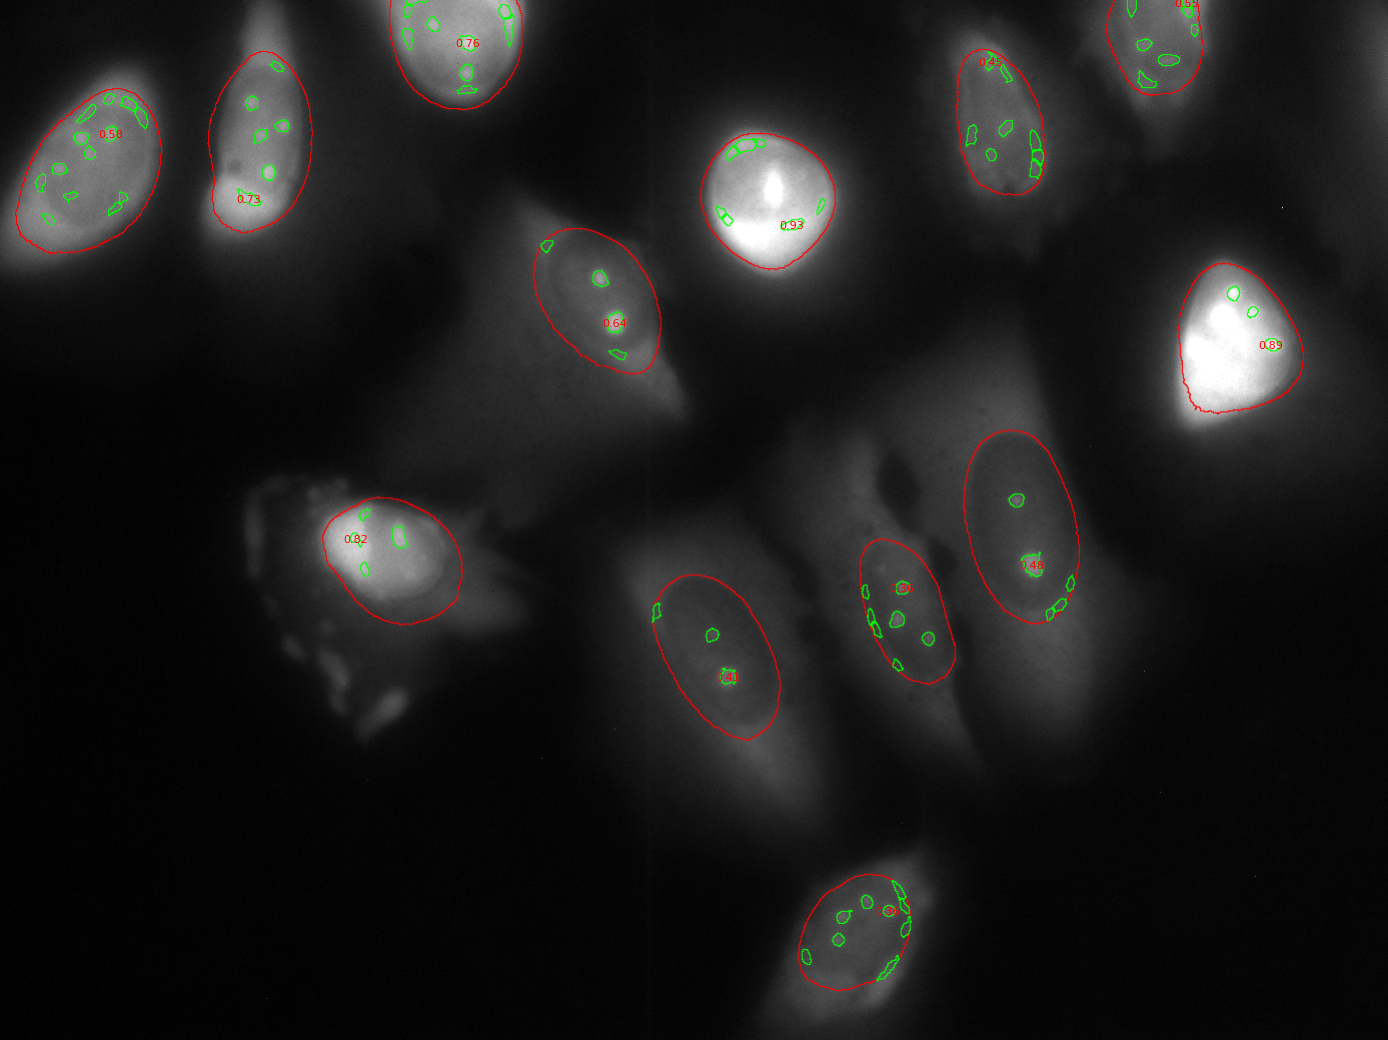
\includegraphics[width=\linewidth]{images/cellprofiler_channel1}
\caption{Example analysis performed with CellProfiler}
\label{fig:cellprofiler_example}
\end{figure}

\newpage
\section{Requirements}\label{sec:requirements}
The application has to meet the following requirements:
\begin{itemize}
  \item \textbf{Reliable nucleoli detection:} Stable and reliable detection of
  nucleoli is the main purpose of the application. Hence, it is supposed to
  detect at least 75\% of the nucleoli CellProfiler can detect. This includes
  a certain degree of stability concerning fuzzy pictures or pictures with
  inequally distributed or diffuse brightnes.
  \item \textbf{Fast analysis:} As the application is tailored to this single
  task, it is expected to detect a suitable amount of nucleoli in only a small
  fraction of the time required by CellProfiler. The topmost time that the
  application may require to complete the analysis of one image is five seconds.
  \item \textbf{Fallback in case of empty nuclei:} Each nucleus is expected to
  containg at least one nucleolus. Yet, this expectation cannot always be
  fulfilled due to potentially damaged nuclei, fuzzy images, or other reasons.
  In this case, the center of the nucleus has to be provided as fallback target.
  \item \textbf{Visualizer:} In order to quickly check the results directly
  after running the analysis and to provide a way to quickly present the results
  to a potential audience, the application has to provide the possibility to be
  configured so that it shows the results as an image. This image has to contain
  all detected neuleoli targets, fallback targets and the regions of interest,
  e.g. the nuclei.
  \item \textbf{Versatility:} Since the appearance of different specimen can
  vary in various ways, all analysis parameters have to be configurable. Among
  others, this includes the minimum and maximum sizes of nuclei and nucleoli.
  The configuration is supposed to be achieved via an understandable,
  interchangeable, text-based file\footnote{Configurable parameters are
  explained in detail in the User's Manual section}.
  \item \textbf{Statistics:} To determine the most suitable parameters for
  different kinds of specimen, another feature may be configured. This
  statistics feature has to include:
  \begin{itemize}
    \item The amount of detected nuclei
    \item The amount of detected nucleoli
    \item Nuclei to nucleoli ratio as percentage
    \item The distance of each detected nucleolus to the center point of the
    containing nuclei and the average distance in pixels
    \item The area of each detected nucleus and the average area in square
    pixels
    \item The area of each detected nucleolus and the average area in square
    pixels
  \end{itemize}
  \item \textbf{Serialization of the results:} All results have to be stored in
  their accordant files in a subfolder \textit{results} of the folder
  containing the original data. The name of each result file has to contain a
  the timestamp indicating the application's execution in the format
  \newline \code{<year>\_<month>\_<day>\_<hour>\_<minute>\_<second>}.
  \newline E.g. \code{targets\_2014\_11\_20\_14\_50\_35.txt}.
  
  In the following, the accordant formats and files are described.
  \begin{itemize}
    \item \textbf{Targets:} Real targets and fallback targets sre to be saved in
    one txt-file named \code{targets\_<timestamp>.txt} in the
    following format:
    \begin{lstlisting}[caption=Format of results txt-file]
# nucleoli targets
<target number> : [<x-coord>, <y-coord>]
...
# targets in center of empty nuclei
<target number> : [<x-coord>, <y-coord>]
...
\end{lstlisting}

\textbf{Example:}
\begin{lstlisting}[caption=Example of results file]
# nucleoli targets
1 : [468, 43]
2 : [1183, 14]
# targets in center of empty nuclei
3 : [87, 174]
4 : [769, 198]
\end{lstlisting}
\item \textbf{Statistics:} The statistics as mentioned above have to be
stored in a txt-file named
\code{statistics\_<timestamp>.txt}. An example of the
statistics file can be found in the appendix.
\item \textbf{Result image:} The image as it would be displayed by the
visualizer has to be stored to a file named

\code{targets\_<timestamp>.<original image filetype>}. See Figure
\ref{fig:target_image_example} for an example the image.
\begin{figure}[h]
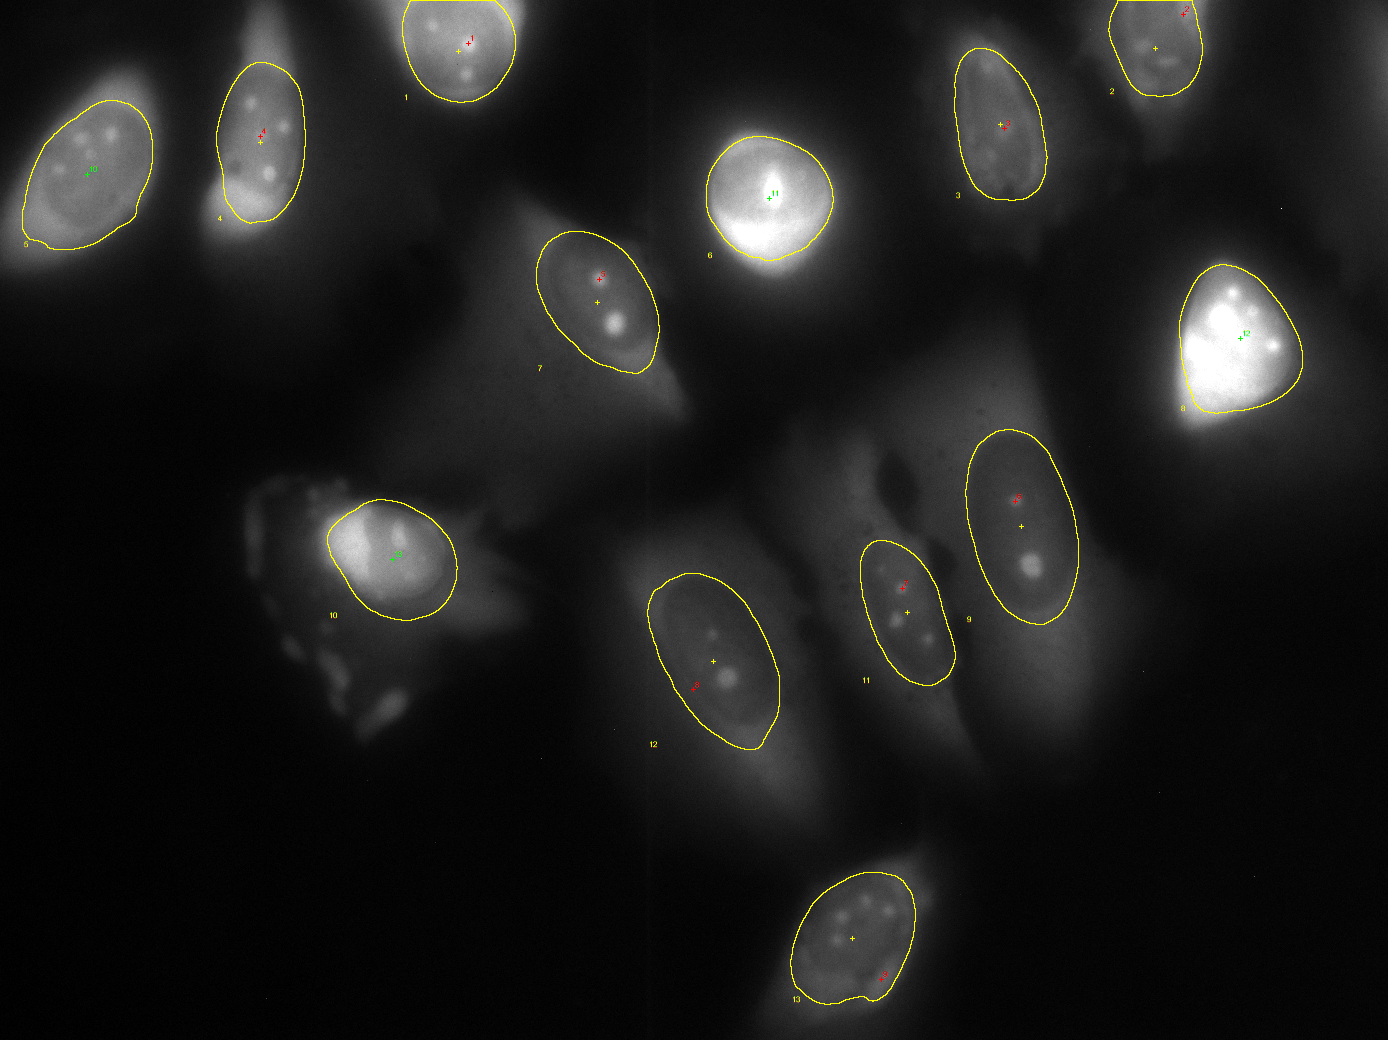
\includegraphics[width=\linewidth]{images/targets_example}
\caption{Example of the image containing the results}
\label{fig:target_image_example}
\end{figure}
  \end{itemize}
  \item \textbf{Quick and easy deployment:} The application is supposed to be
  deployed and run as easily as possible. Since the environment and the machines
  this will happen on may vary drastically, a versatile and independent way to
  do this is required. The Java framework delivers this possibility. Hence, the
  application will be developed using Java.
  \item \textbf{Use of an established graphics framework:} In
  order to keep maintenance effort as small as possible and, in case of
  potential future development, time it takes the developer to familiarize with
  the project, as short as possible, an established and well documented graphics
  framework has to be used. ImageJ meets these requirements and furthermore can
  be easily used as a library within a Java application.
\end{itemize}

\newpage
\section{User's Manual}

\subsection{System Requirements}
The application requires the Java Runtime Environment 1.7 or higher. For
Microsoft Windows 64bit operating system this results in the following minimum
system requirements \footnote{Further details on the system requirements can be
found at:
https://docs.oracle.com/javase/7/docs/webnotes/install/}:

\begin{table}[h]
\centering
\begin{tabular}{ l | r }
Memory: & 128MB \\
\hline
Processor: & Pentium 2 @ 266MHz \\
\hline
Disc space: & 124 MB + 2 MB \\
\end{tabular}
\caption{Minimum system requirements of Java 1.7 on Windows 64bit}
\label{tab:system_requirements_java7}
\end{table}

As it is good practice and vital to the security of any system, the Java
framework should be updated on a regular basis. Note that the requirements may
change with any update.

\subsection{Starting the Application}
Starting the application is acoomplished using the command line interface via
Java's \code{java -jar} or \code{javaw -jar} command\footnote{See
https://docs.oracle.com/javase/7/docs/technotes/tools/windows/java.html for
further details.}. Furthermore, the application expects the configuration file
to be passed as single parameter.

Considering a scenario in which the configuration file (see \ref{sec:configuration}) is
stored as \code{configuration.txt} in the same folder as the \code{NuFi.jar}, the
following command will properly start the application:
\newline\code{java -jar NuFi.jar configuration.txt}.


\subsection{Configuration}\label{sec:configuration}
Configuration of the application is performed using a simple text file
containing the information listed in the following. Note that a missing
parameter will result in a fatal error, preventing the application from properly
working.

A complete example of the configuration file can be found in the appendix.

\subsubsection{General Parameters}
This section contains information on filetypes, source folders and naming
convention of source files.
\begin{itemize}
  \item \textbf{Source folder:} The folder containing the source files (e.g.
  image files) on which the analysis will be based. The source folders are
  expected to be provided as absolut path or relative to \code{NuFi.jar}.
  
  Note that the application expects exactly three files of the type defined as
  channel filetype. If there are more or less than three files of that type, a
  fatal error will occur.
  
  \textbf{Key:}
  \newline \code{source.folder}
  
  \textbf{Examples:}
  \newline \code{source.folder = C:/example/images}
  \newline \code{source.folder = ../../example/images}
  \newline \code{source.folder = example/images}
  
  \item \textbf{Used channels:} Each specimen is photographed three times
  using different colorization. This results in three different images
  referred to as different channels. Channels 1 and 3 are used in the process
  of detecting targets, thus, the correct specification and order of the
  files is vital for image analysis. Position one determines channel 1,
  position 3 determines channel 3. The source folder is scanned for files
  containing these channels determination. If these are not found, the
  application will terminate with a fatal error.
  
  \textbf{Key:}
  \newline \code{used.channels}
  
  \textbf{Examples:}
  \newline \code{used.channels = Kanal1, Kanal2, Kanal3}
  \newline \code{used.channels = channel1, channel2, channel3}
  
  \item \textbf{Channel filetype:} Though using the png-file format is advised,
  the application is built to be able to analyze various image formats. If it
  is necessary to analyze images that are not provided in the png-format, the
  accordant format can be provided using this key.
  
  \textbf{Key:}
  \newline \code{channel.filetype}
  
  \textbf{Examples:}
  \newline \code{channel.filetype = png}
  \newline \code{channel.filetype = jpg}
\end{itemize}
\subsection{General Picture Analysis Settings}
This section contains information of the expected size and shape of nuclei and
nucleoli, as well as the width of the in depth-analysis.

\begin{itemize}
  \item \textbf{Size settings:} Since the size of the nuclei and nucleoli in the
  specimen may vary and since the magnification of the microscope used in taking the
  pictures may also change, the size in the photographs may need to be adapted.
  This can be achieved by giving an average size in sqaure-pixels and the
  minimum and maximum sizes as multiples of that size.
  
  \textbf{Keys:}
  \newline \code{nucleus.average}
  \newline \code{nucleus.min.factor}
  \newline \code{nucleus.max.factor}
  \newline \code{nucleolus.average}
  \newline \code{nucleolus.min.factor}
  \newline \code{nucleolus.max.factor}
  
  \textbf{Examples:}
  \newline \code{nucleus.average = 10000}
  \newline \code{nucleus.min.factor = 0.5}
  \newline \code{nucleus.max.factor = 1.5}
  \newline \code{nucleolus.average = 100}
  \newline \code{nucleolus.min.factor = 0.75}
  \newline \code{nucleolus.max.factor = 1.8}
  
  \item \textbf{Minimum circularity:} This parameter pays respect to the
  variation of the objects in their shape. A value of 1 indicates a perfect
  circle, while a 0 indicates that there are no requirements to the shape of the
  object. Since nuclei typically are elliptical in shape, a value of
  approximatly 0.6 is advised. Nucleoli are typically close to a perfect circle.
  Thus, a value of 0.9 includes most of them while it excludes a variety of
  anomalies and prevents false-positives on nuclei borders.
  
  \textbf{Keys:}
  \newline \code{nucleus.min.circularity}
  \newline \code{nucleolus.min.circularity}
  
  \textbf{Examples:}
  \newline \code{nucleus.min.circularity = 0.6}
  \newline \code{nucleolus.min.circularity = 0.9}
  
  \item \textbf{In-depth width:} This parameter defines the variation in
  thresholding used during in-depth anylsis.
  
  \textbf{Key:}
  \newline \code{indepth.range}
  
  \textbf{Examples:}
  \newline \code{indepth.range = 25}
  \newline \code{indepth.range = 10}
  
\end{itemize}

\subsubsection{Improved Image Detection Parameters}
In the standard setting the application will use the improved image detection
algorithm. In this section, the parameters required for this algorithm can be
defined. These include setting for brightness correction
(\code{<object>.background.blur} and \code{<object>.thresholding.blur}) and the
value used for correcting discrepancies between channel 3 colorization and the
acutal size of nuclei (\code{nucleus.boundary.width}).

\begin{itemize}
  \item \textbf{Brightness correction:}
\end{itemize}

\textbf{Keys:}
\newline \code{nucleus.background.blur}
\newline \code{nucleus.thresholding.blur}
\newline \code{nucleus.boundary.width}
\newline \code{nucleolus.background.blur}
\newline \code{nucleolus.thresholding.blur}

\textbf{Examples:}
\newline \code{nucleus.background.blur = 100}
\newline \code{nucleus.thresholding.blur = 3}
\newline \code{nucleus.boundary.width = 5}
\newline \code{nucleolus.background.blur = 10}
\newline \code{nucleolus.thresholding.blur = 1}


\subsection{Structure of Files and Folders}
\begin{figure}
\centering
\raisebox{-\height}{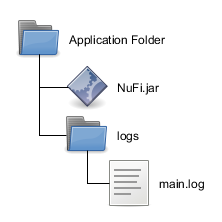
\includegraphics[width=120px]{images/folders_application}}
\raisebox{-\height}{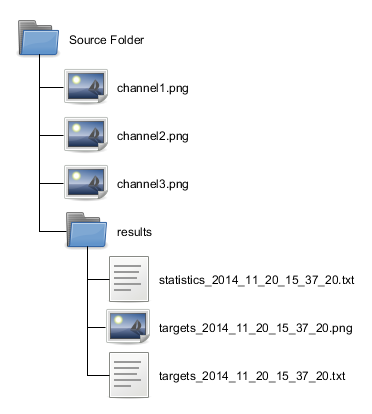
\includegraphics[width=200px]{images/folders_data}}
\caption{Structure of directories and files created in the application's
folder and the source folder}
\label{fig:folders}
\end{figure}

The results of the image analysis will be stored into a directory \code{results}
which is created as a subfolder of the directory defined as source folder. This
directory will contain the targets file, the result image and, in case
statistics are enabled, the statistics file. See figure \ref{fig:folders}.

The application will neither delete nor overwrite files created by a previous
execution since each file contains a timestamp as defined in
\ref{sec:requirements}.

Besides this, the application will create a directory \code{logs} on the same
level as \code{NuFi.bat} is located. This directory contains the log-file of the
application itself. If any unexpected behaviour is encountered while using the
application, refer to this file since it might contain helpful information. See
figure \ref{fig:folders}.

\newpage
\section{Image Analysis}

In this section the procedure of how the application processes and anlyzes
images is explained. Details such as how the applications checks its
configuration are omitted in favor of more emphasis on image analysis.

\begin{figure}[h]
\centering
\begin{subfigure}[b]{0.48\textwidth}
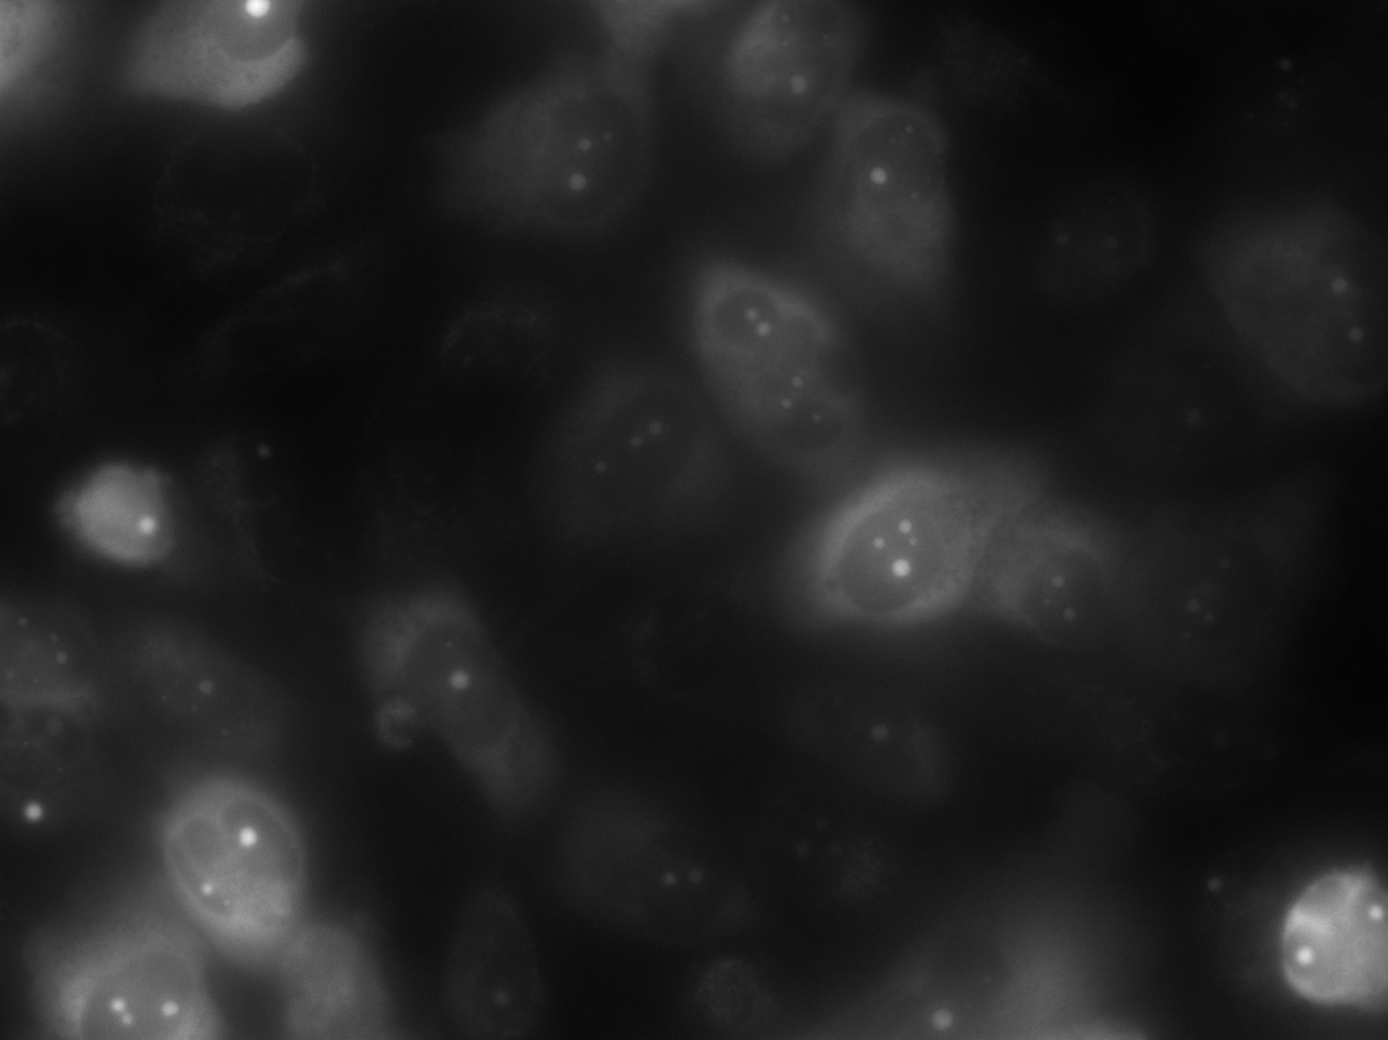
\includegraphics[width=\textwidth]{images/example_Kanal1}
\caption{Channel 1 example image}
\end{subfigure}
\begin{subfigure}[b]{0.48\textwidth}
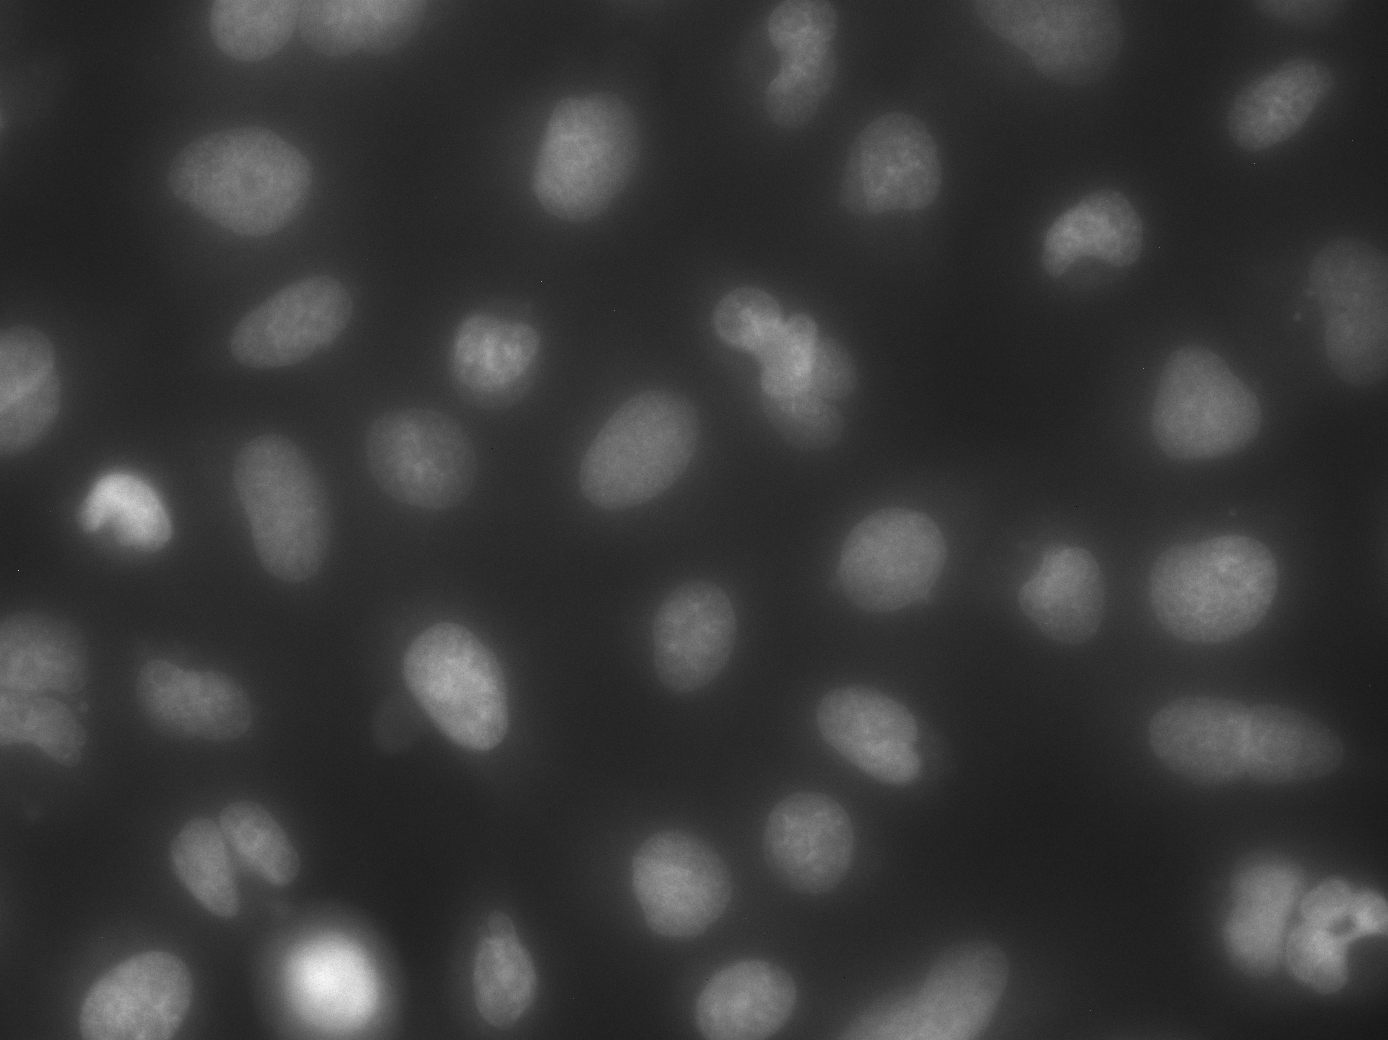
\includegraphics[width=\textwidth]{images/example_Kanal3}
\caption{Channel 3 example image}
\end{subfigure}
\caption{Example images of channel 1 and 3}
\label{fig:example_images}
\end{figure}

\subsection{Target Detection Procedure}
The target detection process can basically devided in two parts. At first, the
regions of interest are detected using channel 3. These regions are then
transferred to channel 1 in order to only analyze those regions that may
actually contain nucleoli.

In the following, these two parts are explained step-by-step using the example
images in figure \ref{fig:example_images}.


\subsubsection{Determining Regions of Interest}
\begin{wrapfigure}{R}{0.33\textwidth}
\vspace{-20pt}

\includegraphics[width=0.3\textwidth]{images/example_Kanal3_gaussian100}
\caption{Channel 3 after Gaussian Blur with a radius of 100 pixels has been
applied}
\label{fig:example_channel3_gaussian}
\vspace{-12pt}
\end{wrapfigure}

Finding the regions of interest is performed using only the image referred to as
channel 3, as this is the image which best shows the nuclei due to the
colorization used.

\begin{wrapfigure}{L}{0.33\textwidth}
\vspace{-12pt}
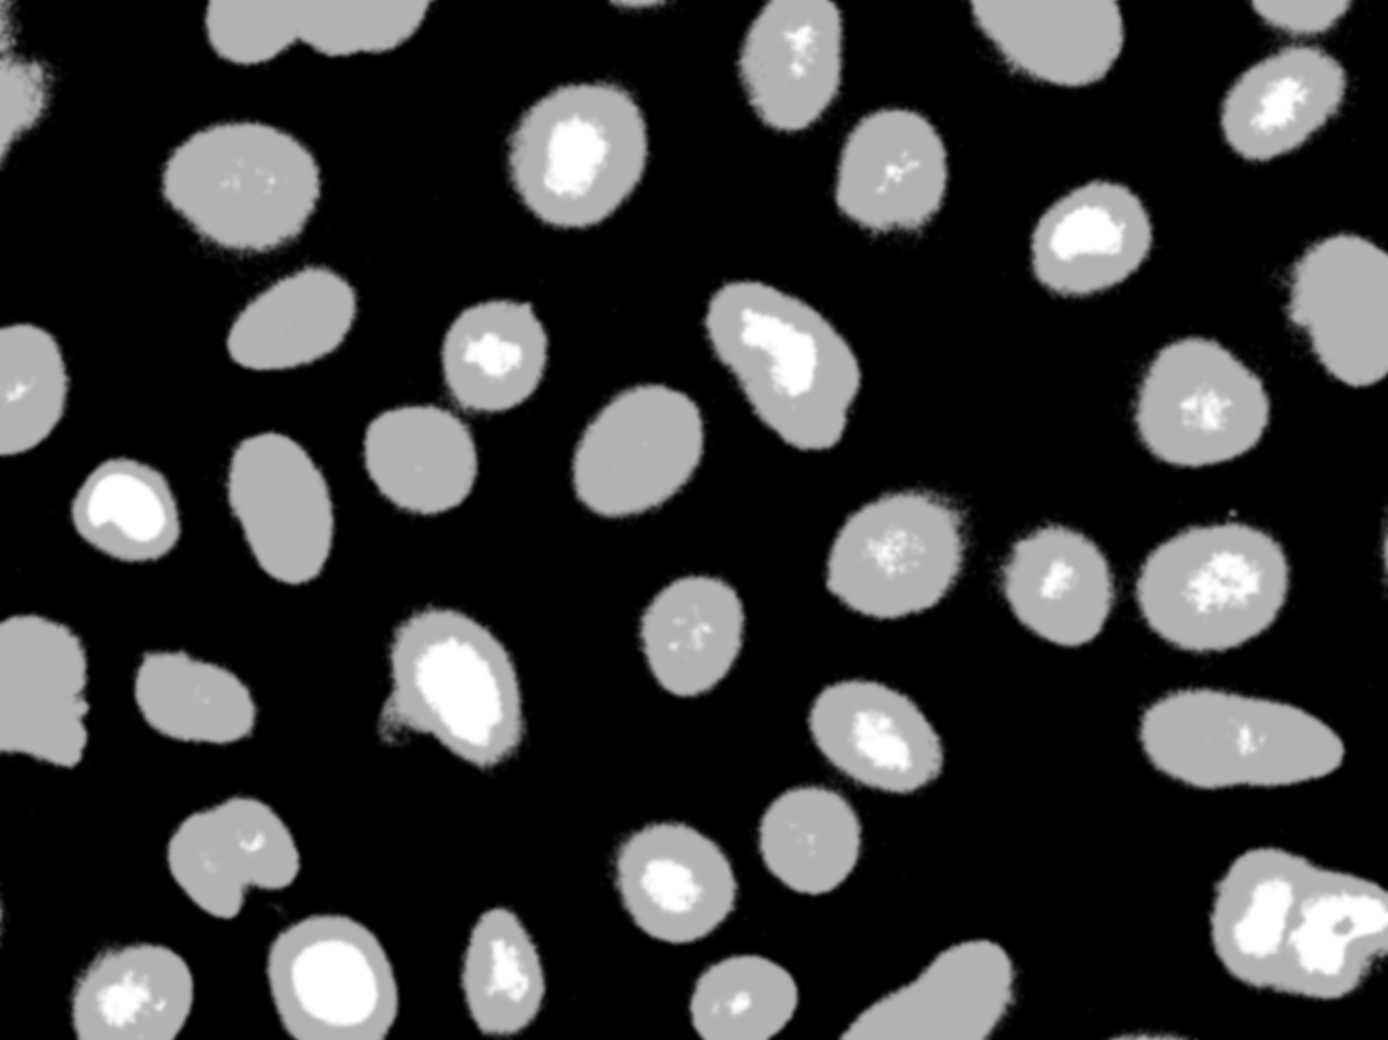
\includegraphics[width=0.3\textwidth]{images/example_Kanal3_multiply178_gaussian2}
\caption{Channel 3 after brightness correction has been performed}
\label{fig:example_channel3_prepared}
\end{wrapfigure}

Typically the images show very uneven exposure to light, resulting in the
necessity of brightness correction as a very first step. This is achieved by
using a gaussian blur with a radius approximately the size of the objects that
are supposed to be found, in this example, a value between 100 and 120 yields
pretty useful results. The result of this operation can be seen in
\ref{fig:example_channel3_gaussian} and is referred to as background image. The
original channel 3 image is then divided by the background image, which means
that each pixel value of the original image is divided by the value of the pixel
of the background image that is at the same location. 
This leads to an image with very small pixel values, typically close to zero,
e.g. the resulting image is all black. Consequently, the next step is to
multiply each pixel value with a constant factor, e.g. 178. As a last step in
this preparation process, a gaussian blur with a small radius, e.g. 2px, is
applied to the image in order to smooth the edges of the nuclei and to reduce
noise. The result of these steps can be seen in \ref{fig:example_channel3_prepared}.

Having finished this preparation, channel 3 now shows evenly distributed
brightness and only little variation in these. This makes the following step,
finding a suitable threshold which is described in detail in
\ref{sec:thresholding}, easier und much more stable across different images.
Figure \ref{fig:channel3_threshold} shows channel 3 after an auto
default threshold was applied.

\begin{wrapfigure}{R}{0.33\textwidth}
\vspace{-12pt}
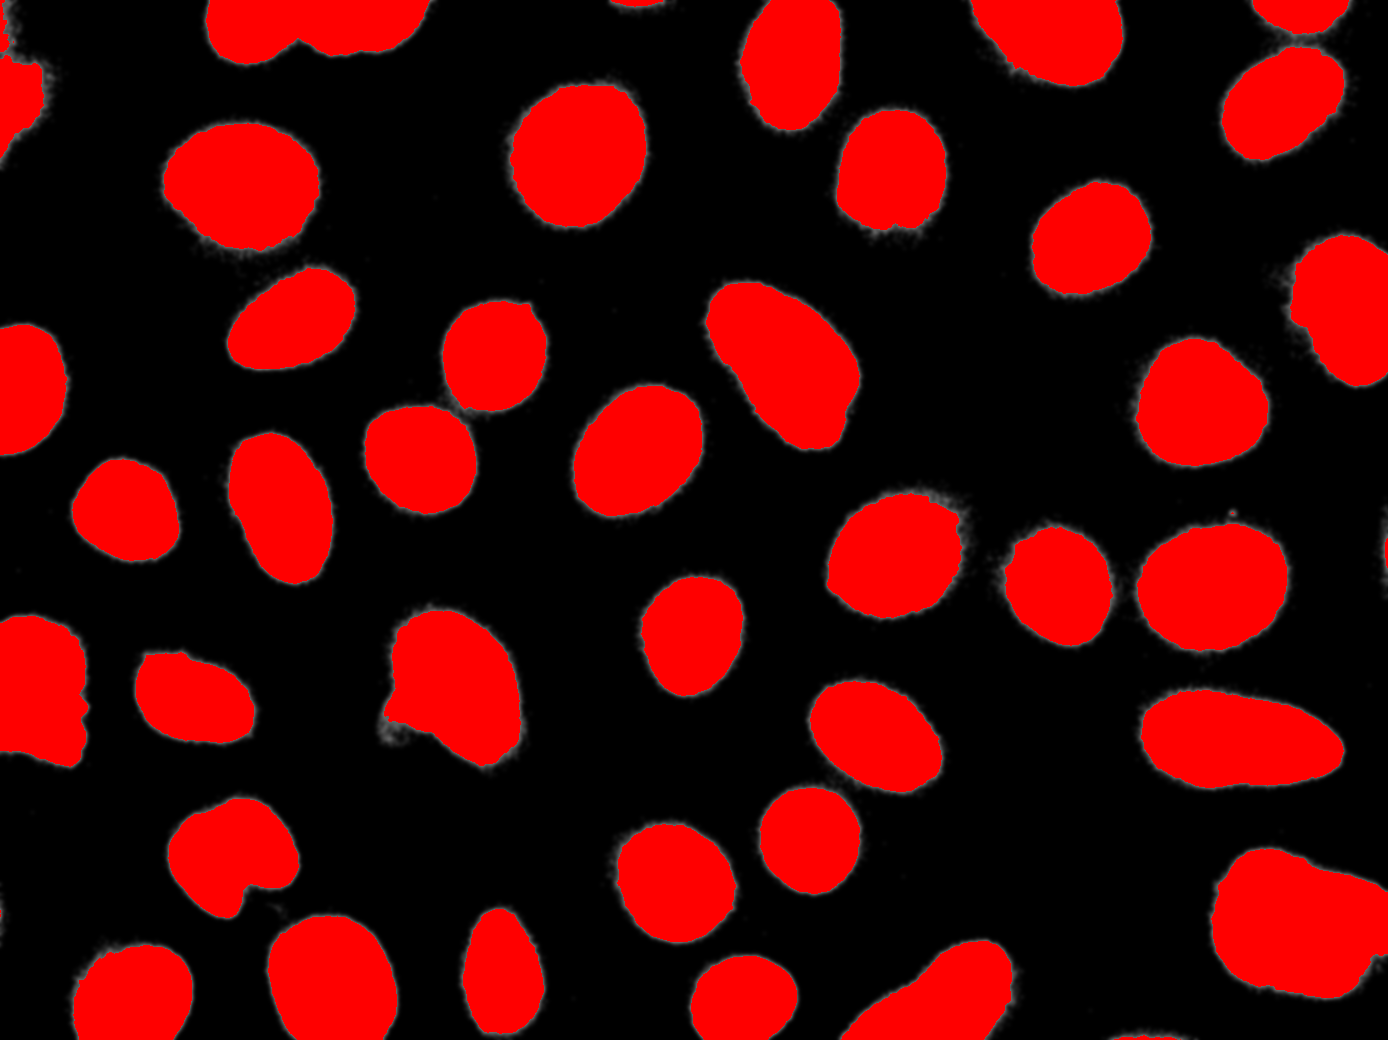
\includegraphics[width=0.3\textwidth]{images/example_Kanal3_corrected_threshold}
\caption{Channel 3 with auto threshold applied}
\label{fig:channel3_threshold}
\end{wrapfigure}

In the last part of determining the regions of interest, the areas to which the
threshold applies, e.g. are marked in red, are analyzed using ImageJ's
Particle Analyzer plugin. Details on how Particle Analyzer works are explained
in \ref{sec:particle_analysis}. Based on configured values for minimum and
maximum area a nucleus may cover and minimum circularity, the regions of
interest are determined. Figure \ref{fig:channel3_rois} shows the result of
running a particle analysis on figure \ref{fig:channel3_threshold} using a
minimum area of 8000 pixel$^2$, a maximum area of 15000 pixel$^2$ and a minimum
circularity of 0.6. Obviously, not all nuclei are recognized as reagions of
interest. In this example, the area of these nuclei are too large or too small.
If the specimen contains a vast amount of too large or too small nuclei,
changing the configured minimum and maximum sizes should be adapted. 

The regions of interest determined in this first part of the image analysis are
the basis of finding nucleoli in the next step. If these regions cannot be
properly determined, for example due to low quality images or flawed
colorization, the subsequent analysis will not yield feasible results.

See appendix for high resoltion versions of the images used in this section.

\begin{figure}[h]
\centering
\fbox{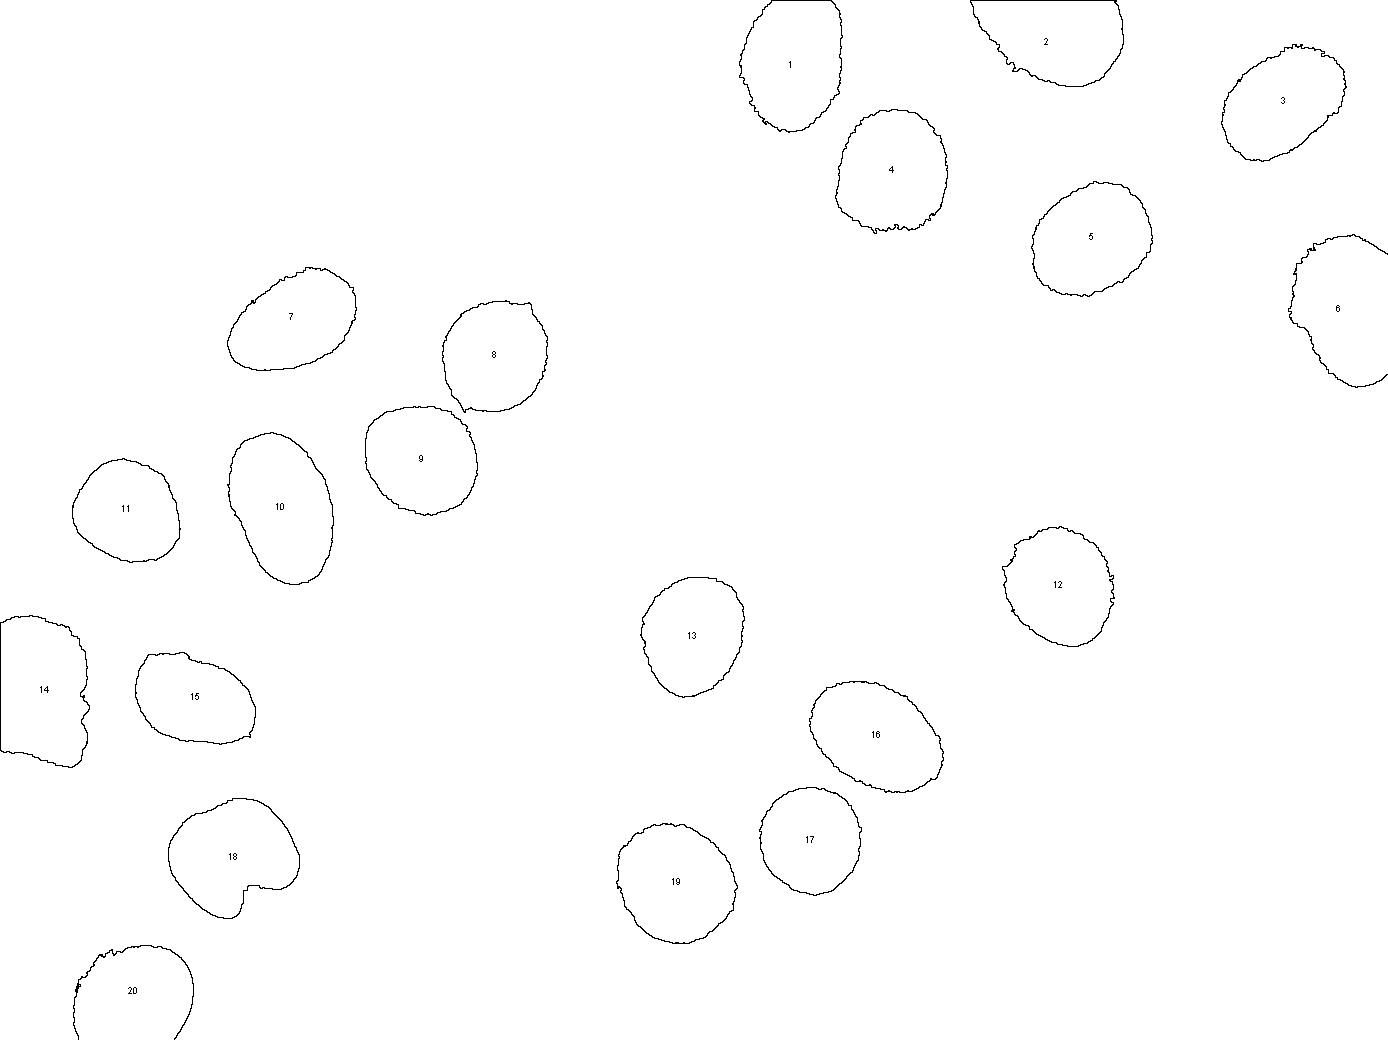
\includegraphics[width=0.8\textwidth]{images/example_Kanal3_rois}}
\caption{Regions of interest found by Particle Analyzer in thresholded channel 3
image}
\label{fig:channel3_rois}
\end{figure}

\subsubsection{Finding Nucleoli}
Having found the regions of interest, the area which has to be searched is
drastically reduced. Furthermore, since each region is analyzed separately,
influence from uneven exposure to light is negligible. Hence, in favor of
faster execution no further brightness correction is performed while detecting
nucleoli. The following describes the process by the example of one region of
interest, e.g. one nucleus. Nonetheless, in the whole process of target
detection, this process is performed for each region of interest. The example
nucleus can be seen in figure \ref{fig:example_nucleus}.

\begin{wrapfigure}{R}{0.33\textwidth}
\vspace{-12pt}
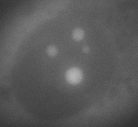
\includegraphics[width=0.3\textwidth]{images/example_nucleus}
\caption{Example nucleus}
\label{fig:example_nucleus}
\vspace{-12pt}
\end{wrapfigure}

The first step in order to analyze a single nucleus is to crop the affected
region as seen in \ref{fig:example_nucleus}. Apparently, the region of interests
border does not exactly match the boundaries of the nucleus. This is caused by
the differences in colorization of channel 1 and 3 and by a delay between taking
the pictures. Furthermore, the colorization of channel 1 causes the boundaries
of nuclei to be nearly as bright as the nucleoli. Without proper correction
false-positives are likely to appear on the boundaries. To counter this, the
extend of the region of interest is shrinked by the configured amount of pixels.
Additionally, in order to prevent the brightness outside the region of interest,
all pixels that are not inside the region, are set to black. This results in the
image depicted in figure \ref{fig:example_nucleus_shrinked_blacked}.

\begin{wrapfigure}{L}{0.33\textwidth}
\vspace{-12pt}
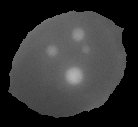
\includegraphics[width=0.3\textwidth]{images/example_nucleus_shrinked8_blacked}
\caption{Region of interest shrinked by 8 pixels, everything outside the region
is set to black}
\label{fig:example_nucleus_shrinked_blacked}
\vspace{-12pt}
\end{wrapfigure}

After preparing the image of the nucleus like this, the analysis is continued by
applying an auto determined threshold using ImageJ's auto thresholding
procedures. In contrast to determining the regions of interest, where all
thresholding methods lead to comparable results, different methods lead to
significantly different results when applied here. Figure
\ref{fig:threshold_comparisson} shows the effects of different thresholding
methods.

By comparing the results of different thresholding methods applied to numerous
nuclei found in several pictures, the MaxEntropy method, depicted in figure
\ref{fig:threshold_maxentropy}, was determined as the most suitable one.

\begin{figure}[h]
\centering
\begin{subfigure}[b]{0.23\textwidth}
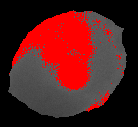
\includegraphics[width=\linewidth]{images/example_nucleus_threshold_default}
\caption{Default}
\end{subfigure}
\begin{subfigure}[b]{0.23\textwidth}

\includegraphics[width=\linewidth]{images/example_nucleus_threshold_huang}
\caption{Huang}
\end{subfigure}
\begin{subfigure}[b]{0.23\textwidth}
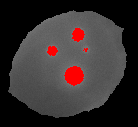
\includegraphics[width=\linewidth]{images/example_nucleus_threshold_maxentropy}
\caption{MaxEntropy}
\label{fig:threshold_maxentropy}
\end{subfigure}
\begin{subfigure}[b]{0.23\textwidth}
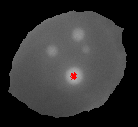
\includegraphics[width=\linewidth]{images/example_nucleus_threshold_shanbhag}
\caption{Shanbhang}
\end{subfigure}
\caption{Comparisson of different thresholding methods}
\label{fig:threshold_comparisson}
\end{figure}

Based on the threshold achieved by using the MaxEntropy method, a particle
analysis is performed similar to the one performed to determine the regions of
interest, but with parameters that pay respect to the size and shape of nucleoli
rather than nuclei. Figure \ref{fig:example_nucleus_shrinked_blacked} shows the
result of an analysis with a minimum size of 80 pixel$^2$, a maximum size of 350
pixel$^2$ and a minimum circularity of 0.8. Note that the nucleolus on the
right is not recognized due to the fact that it is smaller than the configured
minimum size.

\begin{figure}[h]
\centering
\begin{subfigure}[b]{0.23\textwidth}
\fboxsep=0.5mm
\fbox{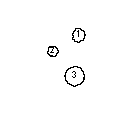
\includegraphics[width=\textwidth]{images/example_nucleus_rois}}
\caption{Plain regions of interest}
\end{subfigure}
\quad
\begin{subfigure}[b]{0.23\textwidth}
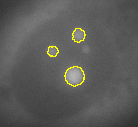
\includegraphics[width=\textwidth]{images/example_nucleus_rois_overlay}
\caption{Regions of interest as overlay}
\end{subfigure}
\caption{Regions of interest found by particle analysis}
\end{figure}

To determine which of the nucleoli found is the most suitable target, the sizes
of all nucleoli within one nucleus are compared. In order to ensure high
accuracy during exposure to radiation later on in the process of analyizing the
specimen, the largest nucleolus, e.g. covers the largest area, is chosen. Note
that this will not result in choosing too large objects, since these are ignored
due to the maximum size defined in particle analysis. In the example nucleus,
region 3 is determined the most suitable choice, which can bee seen in figure
\ref{fig:example_nucleus_target}. 

\begin{figure}
\centering
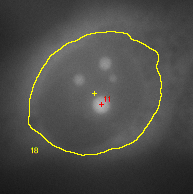
\includegraphics[width=0.3\textwidth]{images/example_nucleus_target}
\caption{Extract from the result image showing the example nucleus and
the chosen target}
\label{fig:example_nucleus_target}
\end{figure}

\subsection{Thresholding}\label{sec:thresholding}
Despite the possibility of determining the threshold by hand or, respectively
newly implement ways of automatically finding a suitable threshold, the
application relies on ImageJ's AutoThresholder. This ImageJ plugin provides the
possibility to use different methods to determine the threshold automatically.
These include methods such as Huang \cite{huang93}, Otsu

\subsection{Particle Analysis}\label{sec:particle_analysis}

\newpage
\section{Conclusion and Prospect}

\subsection{Conclusion}

\subsection{Prospect}


\newpage
\addcontentsline{toc}{section}{Bibliography}
\bibliography{sources}

\end{document}